\documentclass[twoside,12pt]{report}
\usepackage[T1]{fontenc}
\usepackage[utf8]{inputenc}
\usepackage{amsmath,amssymb,amsfonts}
\usepackage[polish]{babel}
\usepackage{graphicx}
\usepackage{pdfpages}
\usepackage{hyphenat}
\usepackage{txfonts}
\usepackage{hyperref}
\usepackage{float}
\usepackage{listings}
\usepackage{caption}
\usepackage{fancyhdr}
\usepackage{indentfirst}
\usepackage{geometry}
\usepackage{verbatim}
\usepackage{parskip}

\geometry{a4paper,left=35mm,right=25mm,top=25mm,bottom=25mm}

\renewcommand{\headrulewidth}{0.1pt}
\renewcommand{\chaptername}{Rozdział}
\renewcommand{\contentsname}{Spis treści}
\renewcommand{\figurename}{Rys.}
\renewcommand{\tablename}{Tab.}
\renewcommand{\lstlistingname}{Listing}
\renewcommand{\listfigurename}{Spis rysunków}
\renewcommand{\listtablename}{Spis tabel}
\renewcommand{\lstlistlistingname}{Spis listingów}
\renewcommand{\bibname}{Bibliografia}

\pagestyle{fancy}
\fancyhf{}
\fancyhead[LE,RO]{\rightmark}
\fancyfoot[LE,RO]{\thepage}
\setlength{\headheight}{15.13202pt}
\setlength{\parindent}{1.5em}
\setlength{\emergencystretch}{3em}

\newtheorem{definition}{Definicja} % przykład nowego środowiska 
\newtheorem{example}{Przykład}[chapter] % przykład nowego środowiska 
\newtheorem{corollary}{Wniosek}[chapter] % przykład nowego środowiska 

\begin{document}


\includepdf[pages={1,2}]{titlepage.pdf}

\tableofcontents	% generuje spis treści ze stronami !!!

\chapter{Wstęp.} \label{rozdz.wstep} 

\section{Problematyka i zakres pracy.}

Niniejsza praca obejmuje zagadnienia z zakresu inżynierii oprogramowania i sztucznej inteligencji. Głównym jej celem jest stworzenie aplikacji optymalizującej strukturę sieci drogowej.

Problemy komunikacji w dzisiejszych miastach są wszystkim znane. Zatory drogowe i korki w godzinach szczytu są chlebem powszednim. Pomimo wielu prób i sposobów, wciąż nie istnieje metoda jednoznacznie rozwiązująca tę kwestię. Bezspornie, dotyczy to wszystkich miast na świecie. Z teoretycznego punktu widzenia, jedynym rozwiązaniem jest komunikacja publiczna. Oczywistym jest jednak, że nigdy nie doprowadzimy do sytuacji, gdy wszyscy mieszkańcy zrezygnują ze swoich pojazdów. Dodatkowo, wiele osób i usług wymaga oddzielnej formy transportu. W obliczu tych faktów miasta decydują się na rozwój swojej infrastruktury drogowej. Budowa nowych tras oraz poszerzanie starych przynosi nadzieję mniejszych zatorów a co za tym idzie, szybszego przejazdu do celu. Niestety, historia pokazuje, że takie inwestycje nie zawsze przynoszą oczekiwane korzyści.

Teorii próbujących wytłumaczyć te zjawiska, jak również dowodów, które je popierają lub obalają jest wiele. Jedną z najpopularniejszych oraz taką która została wykorzystana w niektórych miastach na świecie jest paradoks Braessa\cite{braess}. Jest to twierdzenie matematyczne orzekające, że w pewnym modelu ruchu drogowego czasy podróży pojazdów mogą ulec wydłużeniu po dodaniu do sieci drogowej nowego połączenia. Ma ono również  zastosowanie w przypadku  sieci komputerowych oraz istnieją jego analogie dla doświadczeń fizycznych.

Moim celem jest opracowanie metody, która dla danej struktury sieci drogowej zmodyfikuje ją wykorzystując prawidłowość z powyższego paradoksu. W efekcie poprzez zamknięcie wybranych ulic w danej sieci drogowej, średni czas podróży powinien ulec skróceniu.

\section{Metoda badawcza.}
\subsubsection{Studia literaturowe.}
Moje badania rozpocząłem od poszukiwania źródeł traktujących o opisywanym przeze mnie problemie. Paradoks Braessa został sformułowany w 1970 roku i był od tego czasu wykorzystywany przy planowaniu przestrzeni i infrastruktury wielu miast, np:

\begin{itemize}
\item Korea, Seul, likwidacja m.in. estakad Cheonggyecheon,
\item Niemcy, Stuttgart, likwidacja dróg zbudowanych w latach 60,
\item USA, Nowy Jork, czasowe zamknięcie ulicy 42,
\item USA, Winnipeg.\cite{urban}
\end{itemize}  

\subsubsection{Propozycja rozwiązania problemu.}
Oczywistym rozwiązaniem problemu komunikacji mogłoby być stworzenie idealnej sieci odpowiadającej potrzebom danego miasta. Rozbudowa lub modyfikacja tej infrastruktury jest jednak kosztowna i czasochłonna. Dlatego zdecydowałem się na przetestowanie rozwiązania zaproponowanego przez Braessa. Ponieważ istnieją prace negujące lub podważające paradoks\cite{newinsights} , zdecydowałem by przy potwierdzaniu wyniku optymalizacji nie kierować się wyłącznie założeniami zawartymi w twierdzeniu.

\subsubsection{Opis zastosowania algorytmów genetycznych.}
Ponieważ nie znalazłem żadnych przesłanek wykazujących jednoznaczną ocenę co do słuszności zamknięcia danej ulicy, zdecydowałem się losowe przeszukiwanie przestrzeni rozwiązań. Jednym z rozwiązań w przypadku takich poszukiwań są algorytmy genetyczne, na które się zdecydowałem w swojej pracy.

\subsubsection{Przedstawienie oceny optymalizacji.}
Paradoks Braessa zakłada dość oczywiste potwierdzenie swojej wiarygodności. Zdecydowałem się więc na zastosowanie zewnętrznego systemu oceny. Taką rolę spełniają systemy symulacji. System, który wybrałem działa zupełnie oddzielnie od metody twierdzenia, symulując rzeczywisty ruch na danej sieci drogowej. Wynik symulacji jest jednoznaczną wartością liczbową, przedstawiającą średni czas przejazdów wszystkich agentów biorących udział w danym scenariuszu. Zakładając stały zestaw agentów dla zmieniających się w wyżej opisany sposób sieci, dążymy oczywiście do minimalizacji średniego czasu przejazdu.

\subsubsection{Ocena możliwości wdrożenia proponowanych rozwiązań.}
Paradoks Braessa nie jest jedynym twierdzeniem traktującym o problemach komunikacyjnych miast. Wiele teorii jest opartych głownie na socjologicznych lub psychologicznych założeniach\footnote{np. paradoks Downsa-Thomsona\cite{downs} czy prawo Lewisa-Mogridge’a\cite{lewis}}
. Są jednak niemniej ważne.
Biorąc pod uwagę złożoność problemu, wynik otrzymany podczas eksperymentu nie może być dowodem ani decydującym głosem w decyzjach dotyczących ustalaniu rzeczywistego ruchu drogowego miasta. 


\section{Przegląd literatury w dziedzinie.}
Rozszerzyć odpowiedni podpunkt z metody badawczej, np. wg podziału:
\subsubsection{Źródła książkowe polskojęzyczne i tłumaczenia.}
\subsubsection{Źródła książkowe obcojęzyczne.}
\subsubsection{Artykuły naukowe, raporty z badań, komunikaty konferencyjne,
dokumentacje techniczne, manuale, instrukcje}
\subsubsection{Źródła elektroniczne.}


\section{Układ pracy.}
Tematem pracy jest: ....., zaś za główny cel przyjęto ...... . 
Rozdział \ref{rozdz.wstep} zawiera wstęp i cele pracy. W rozdziale drugim
opisano/...... w Rozdziale 3. zawarto............ Rozdział 4. przedstawia..... 
W podsumowaniu pracy przedstawiono..........................., z czego wynika,
że ................  
Najważniejszym wnioskiem/wynikiem/rezultatem pracy jest.................. {\bf wyraźnie określić
CO TO JEST}. 

{\bf cały podrozdział ok. 1 strony}.



\chapter{Optymalizacja struktury sieci drogowej.}
\section{Podstawowe definicje.}
Ten podrozdział powinien zawierać dokładny opis terminologii  pojęć zasadniczych dla tematu pracy, którymi autor będzie się posługiwał przy realizacji głównych celów pracy. 


\begin{definition}\label{Sieć drogowa}
Co chce to powiem
\end{definition}


\begin{figure}[ht]
\begin{center}
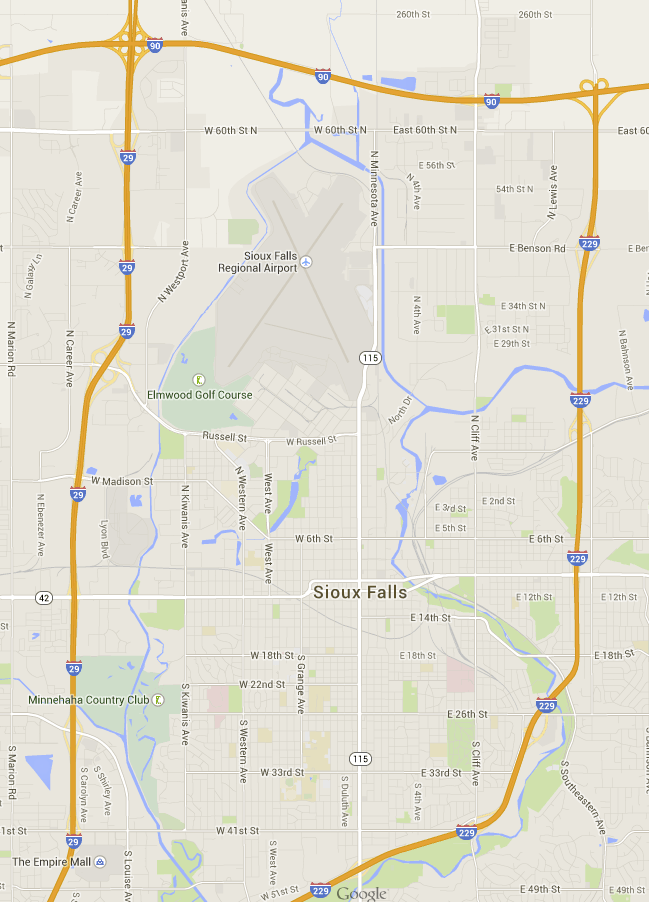
\includegraphics[width=0.30\textwidth]{img/siec}
\caption{Fragment sieci drogowej w Sioux Falls, Południowa Dakota.} 
\end{center}
\end{figure}


\begin{definition}\label{Sieć drogowa w postaci grafu}
Co chce to powiem
\end{definition}


\begin{figure}[ht]
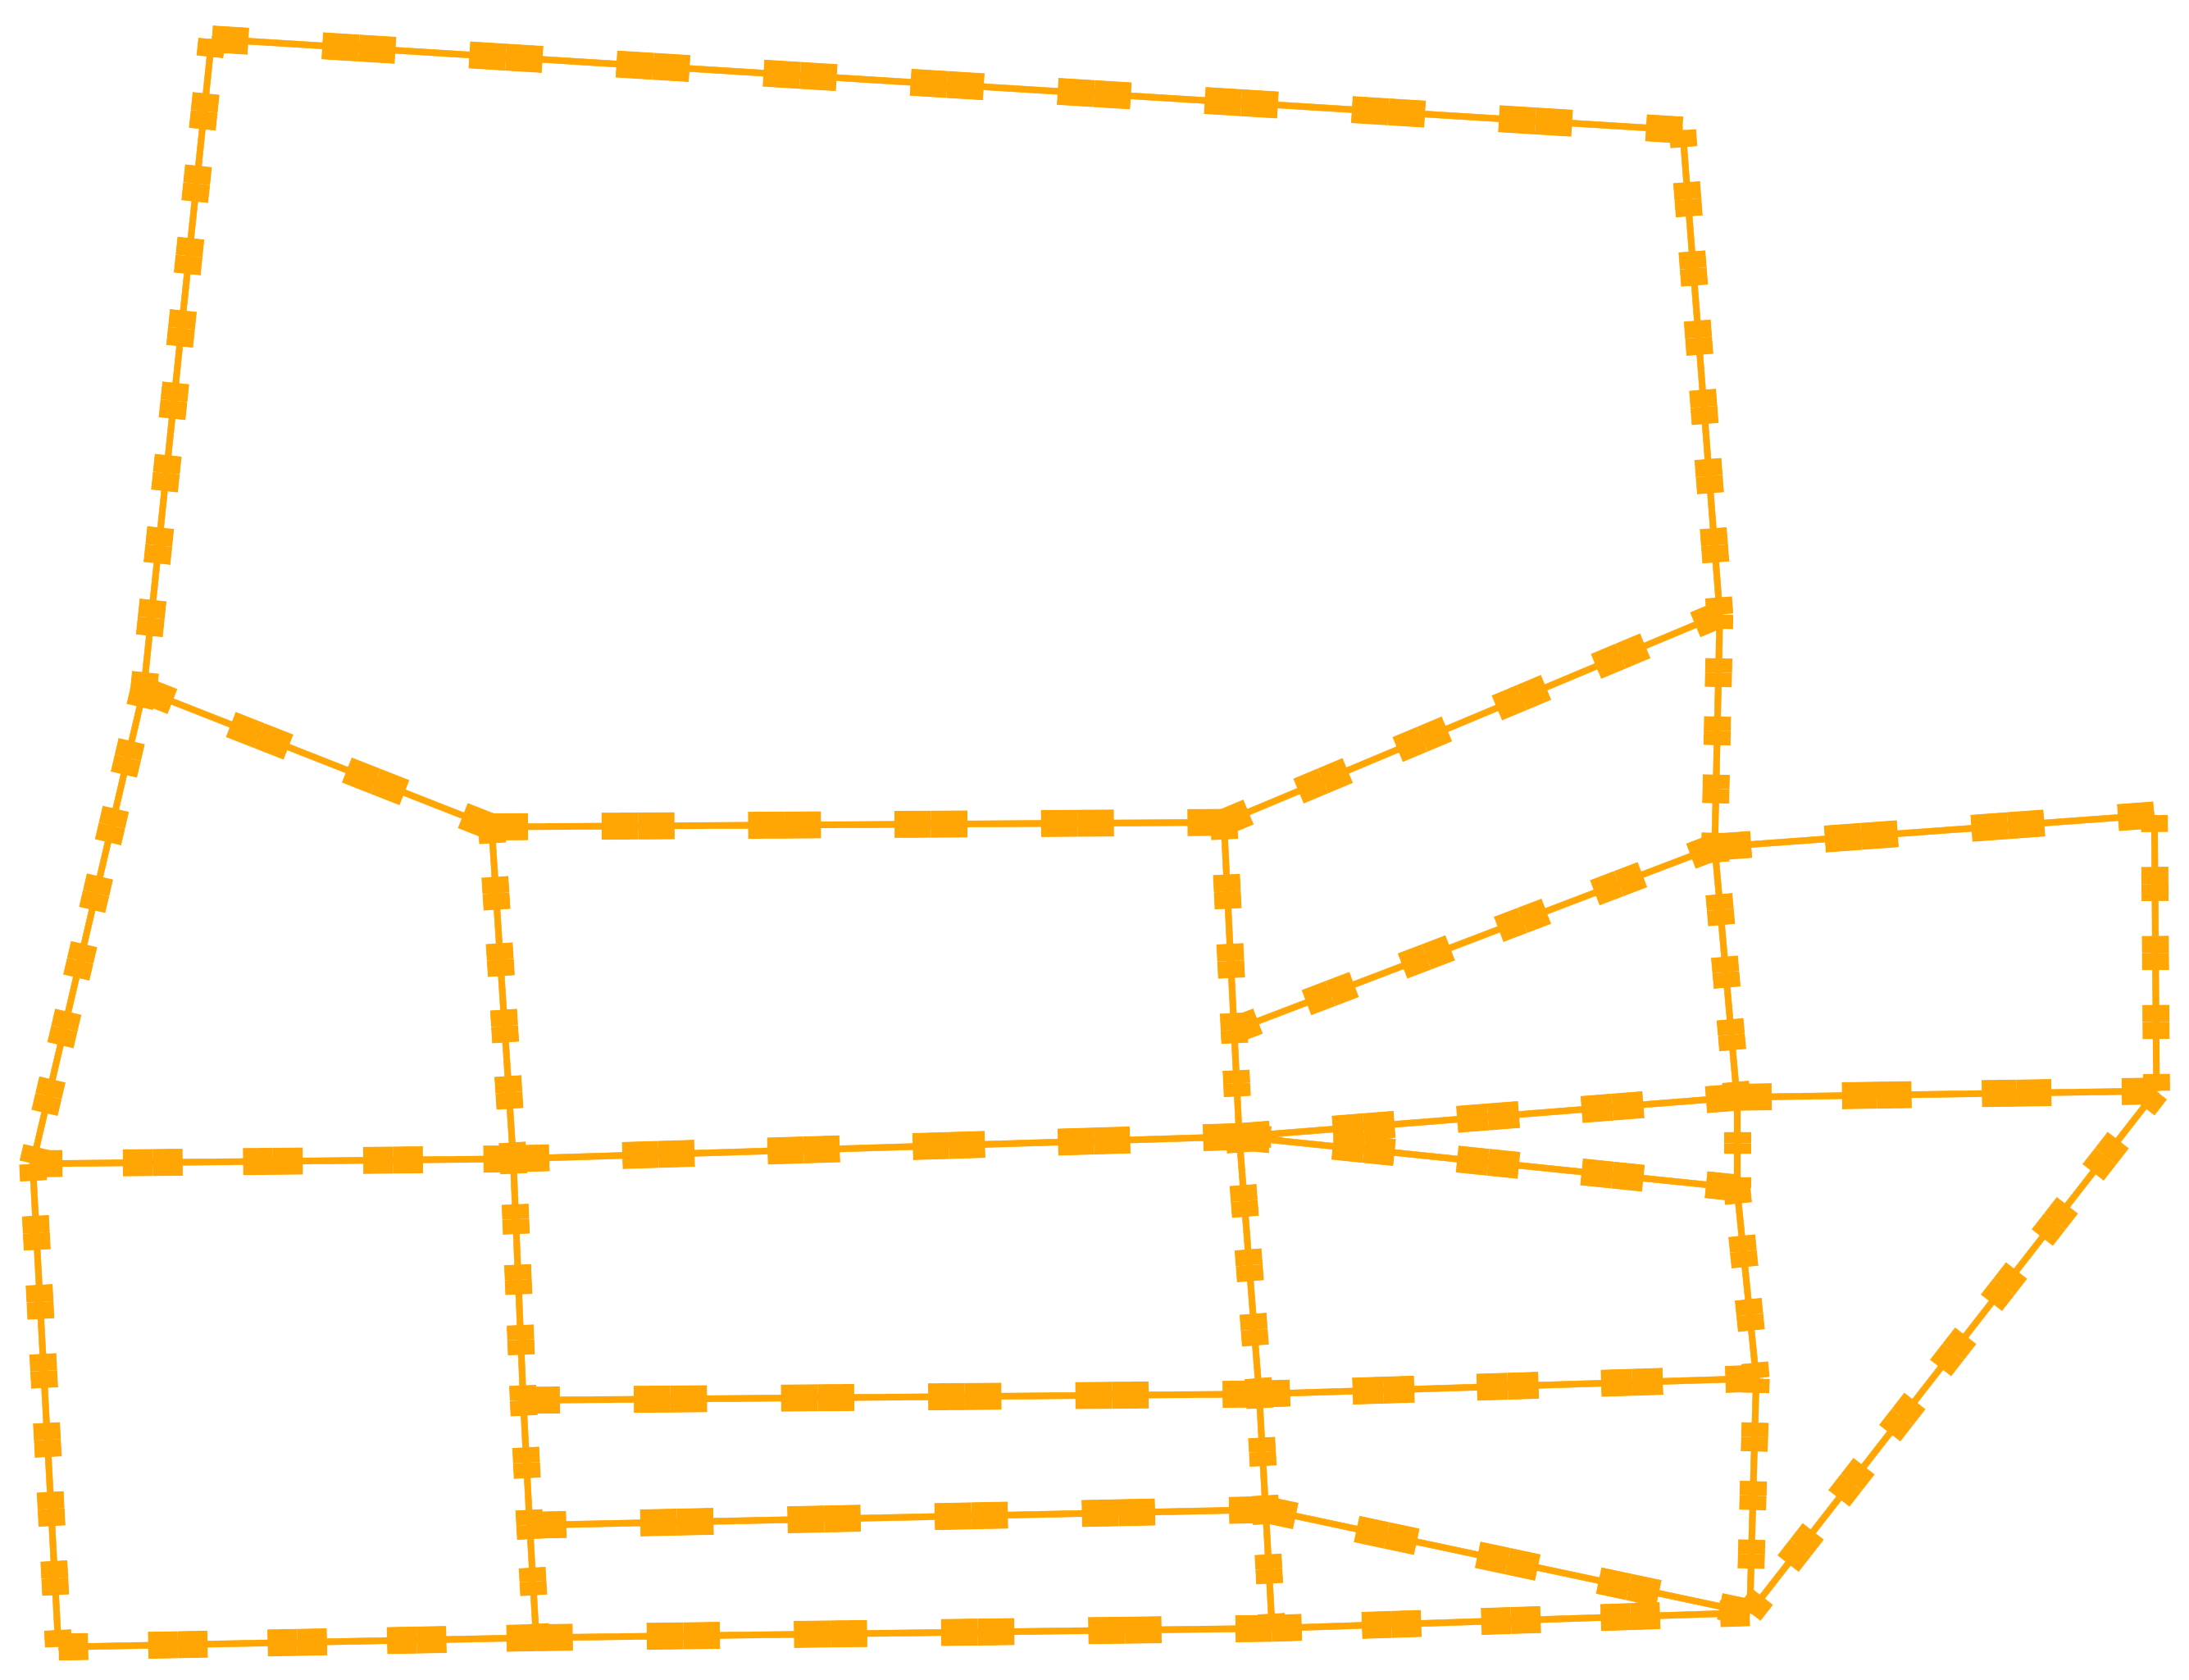
\includegraphics[width=0.55\textwidth]{img/graf}
\caption{Siec drogowa miasta Sioux Falls w postaci grafu.} 
\end{figure}

\begin{figure}[ht]
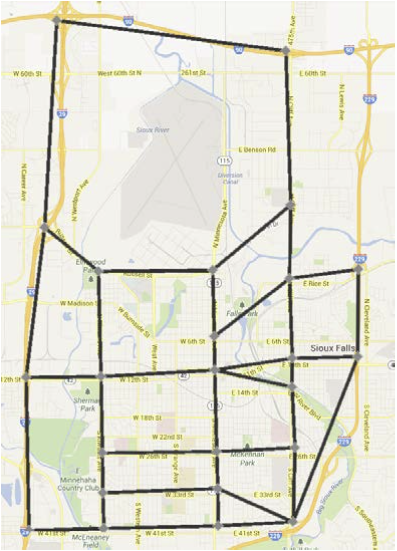
\includegraphics[width=0.38\textwidth]{img/dopasowanie}
\caption{Graf z dopasowaną geometrią \cite{siux}.}
\end{figure}

\section{Paradoks Braessa.}


\begin{figure}[ht]
\centering
\begin{minipage}{.48\textwidth}
\centering

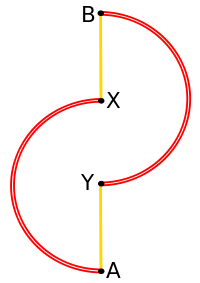
\includegraphics[width=0.7\textwidth]{img/braess1}
\caption{Wyjściowy układ drogowy}

\end{minipage}\hfill
\begin{minipage}{.48\textwidth}
Autostrady:
AX, $t_{AX}(p) =  50 + p$ min
YB, $t_{YB}(p) =  50 + p$ min

Drogi lokalne:
AY, $t_{AY}(p) =  10p$ min
XB, $t_{XB}(p) =  10p$ min

Aut jest 6000 i wszystkie mają za zadanie przejechać trasę z A do B.
\end{minipage}\hfill
\end{figure}


Równowaga Nasha to taka sytuacja, w której każdy z samochodów spowoduje wydłużenie swojego czasu jazdy, zmieniając decyzję co do wyboru trasy przy niezmienionych decyzjach pozostałych aut.
\newline\newline
Jeśli p i q to liczby aut w tysiącach pokonujących odpowiednio trasy AXB i AYB, otrzymujmy równania:

\begin{center}
$p+q = 6 $
$t_{AX}(p)+t_{XB}(p) = t_{AY}(q) + t_{YB}(q)$
$50+p+10p = 10q+50+q$
\end{center}
rozwiązaniem jest $p=q=3$.
Przy tej gęstości ruchu pokonanie obu dostępnych tras zabiera $50+3+30=83$ minuty.



\begin{figure}[ht]
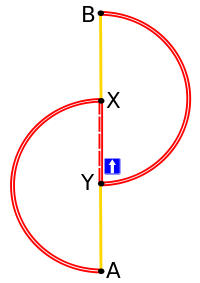
\includegraphics[width=0.7\textwidth]{img/braess2}
\caption{Uzupełniony układ drogowy}
\end{figure}

Do wyjściowego układu drogowego dodana zostaje autostrada:

YX, $t_{YX}(p) =  10 + p$ min

Aut jest nadal 6000 i wszystkie mają za zadanie przejechać trasę z A do B.



Jeśli p, q i r to liczby aut w tysiącach pokonujących odpowiednio trasy AXB, AYB i AYXB, otrzymujmy równania:

\begin{center}
$p+q+r = 6 $
$t_{AX}(p)+t_{XB}(p+r) = t_{AY}(q+r) + t_{YB}(q) = t_{AY}(q+r)+t_{YX}(r)+t_{XB}(p+r)$
\newline
$50+p+10(p+r) = 10(q+r)+50+q = 10(q+r)+ 10 + r + 10(p+r)$
\end{center}
rozwiązaniem jest $p=q=r=2$.
Czas przejazdu każdej z tych dróg wynosi wówczas $50+2+10(2+2)=92$ minuty.

\section{Składowa silnie spójna.}


\section{Punkty artykulacji grafu.}


\section{Klasyczny algorytm genetyczny.}


\begin{figure}[ht]
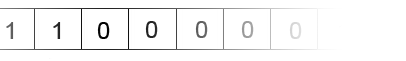
\includegraphics[width=\textwidth]{img/bool}
\caption{Fragment sieci w postaci tablicy binarnej }
\end{figure}

\begin{figure}[ht]
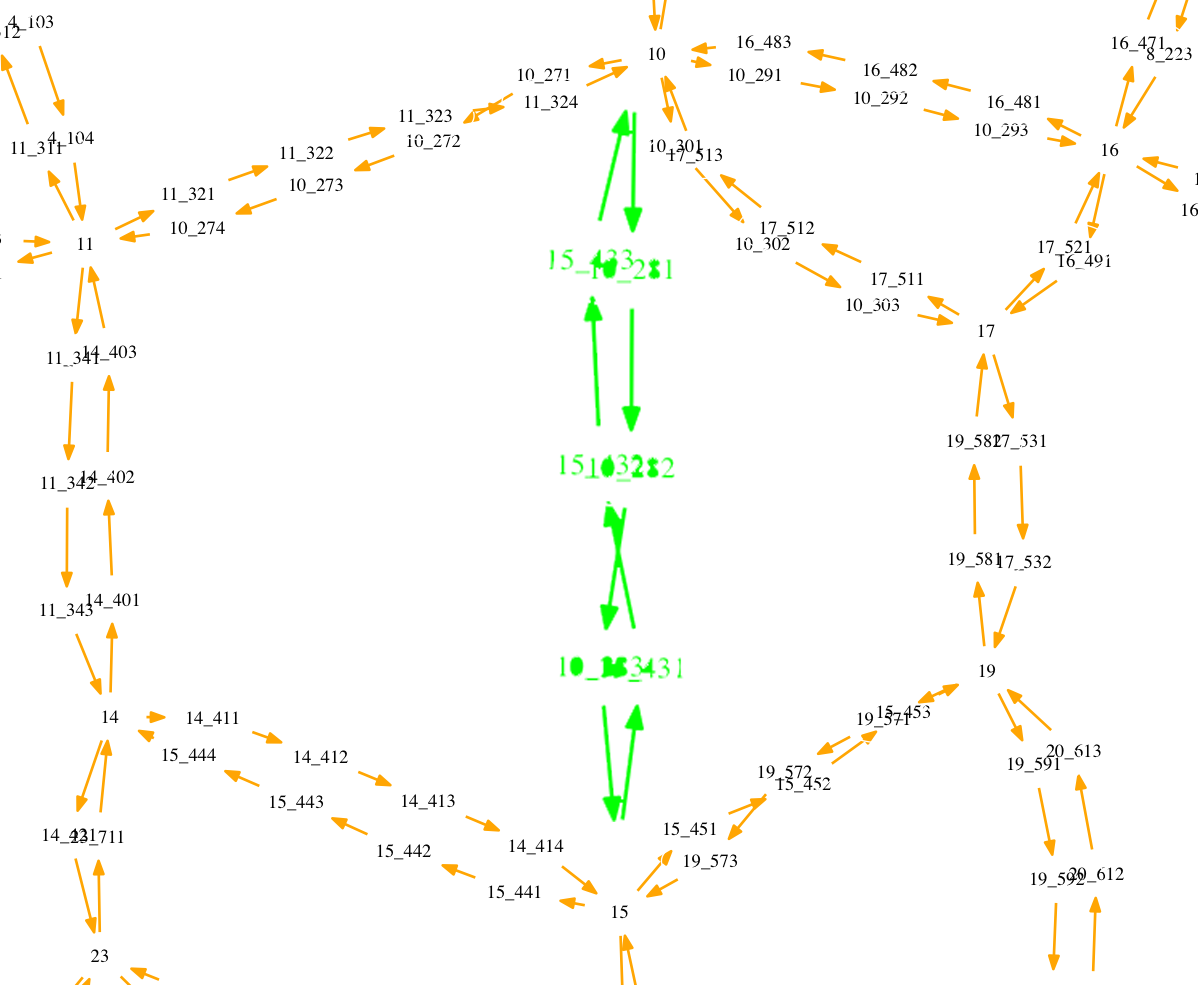
\includegraphics[width=\textwidth]{img/bool-efect}
\caption{Fragment sieci w postaci grafu}
\end{figure}


\chapter{Technologie i metody użyte.}
\section{Symulator transportu.}


\begin{figure}[ht]

\includegraphics[width=0.40\textwidth]{img/matsim}
\caption{Logo symulatora transportu MATSim \cite{matsim}} 
\end{figure}





\section{Przestrzeń poszukiwań.}

Najlepszego rozwiązania będę poszukiwał wykorzystując klasyczny algorytm genetyczny.

\begin{figure}[ht]

\includegraphics[width=0.40\textwidth]{img/math}
\caption{Logo biblioteki Apache Commons Math \cite{math}} 
\end{figure}



\section{Technologie i metodologie programistyczne.}

\begin{figure}[ht]

\includegraphics[width=0.7\textwidth]{img/java}
\caption{Logo Java\cite{java}}
\end{figure}
\begin{figure}[ht]

\includegraphics[width=0.7\textwidth]{img/eclipse}
\caption{Logo IDE Eclipse\cite{eclipse}}
\end{figure}


\begin{figure}[ht]

\includegraphics[width=0.7\textwidth]{img/py}
\caption{Logo Python\cite{python}}
\end{figure}
\begin{figure}[ht]

\includegraphics[width=0.55\textwidth]{img/pydev}
\caption{Logo PyDev\cite{pydev}}
\end{figure}

\section{Zastosowany przykład, Siouxfalls.}


\chapter{Opis projektu.}
Ta część pracy może być podzielona na więcej rozdziałów, np kiedy autor chce
w~szczególności podkreślić któryś z etapów projektu. W zależności od tematu i~celów pracy, pewne sekcje można dodać (np. przy projektowaniu sieci, instalacji
i~konfiguracji serwerów usług sieciowych), inne zaś pominąć.

\section{Dane wejściowe.}


\lstset{
    language=xml,
    tabsize=3,
    rulesepcolor=\color{gray},
    keywordstyle=\color{blue}\bf,
    stringstyle=\color{red},
    breaklines=true,
    basicstyle=\ttfamily\scriptsize}
\lstinputlisting[language=Xml]{img/config.xml}


\section{Wdrożenie.}

\begin{figure}[ht]

\includegraphics[width=0.4\textwidth]{img/trisquel}
\caption{Logo Trisquel\cite{trisquel}}
\end{figure}

pewnie brakuje tekstu

\section{Przewidywane problemy.}

\begin{itemize}
\item Brak gwarancji lepszego wyniku
\item Długi czas obliczeń
\item Duże wymagania dotyczące zasobów
\end{itemize}


\chapter{Podsumowanie.}
\section{Dyskusja wyników.}
Dzięki zrealizowaniu pracy poprawie uległa wydajność ....... Ponadto, o ??
skrócony został czas ........, a koszty osiągnięcia zamierzonego efektu zostały
zmniejszone z ???pln do ???pln za godzinę/ dzień/ jednostkę sprzętu.........
\indent Które cele pracy udało sie zrealizować? co z tego wynika? Które cele
pracy pozostały niezrealizowane i dlaczego? 

\section{Ocena możliwości wdrożenia.}
... ich wartość praktyczna, lokalne i globalne możliwości zastosowania, kwestia
praw autorskich do powstałych produktów, itp. 

\section{Perspektywy dalszych badań w dziedzinie.}
Jak można kontynuować tę pracę, zwłaszcza pod kątem studiów
uzupełniających magisterskich i/lub doktoranckich. Co jeszcze powinno być
zrobione lub ulepszone? Co należy zmienić lub poprawić w pracy z dzisiejszego punktu widzenia?



\addcontentsline{toc}{chapter}{Spis rysunków} 
\listoffigures

\addcontentsline{toc}{chapter}{Spis tabel} 
\listoftables

\addcontentsline{toc}{chapter}{Spis listingów}
\lstlistoflistings

\addcontentsline{toc}{chapter}{Bibliografia} 
\begin{thebibliography}{99}
\bibitem{investigation} 
	Leslie Arthur Keith Bloy, 
	\newblock \textit{An investigation into Braess’ paradox}, 02/2007

\bibitem{newinsights}
	Rric Pas and Shari Principio
	\newblock \textit{Braess’ paradox: Some new insights}, April 1996

\bibitem{conference} 
	Wataru Nanya, Hiroshi Kitada, Azusa Hara, Yukiko Wakita, Tatsuhiro Tamaki, and Eisuke Kita
	\newblock \textit{Road Network Optimization for Increasing Traffic Flow}
	\newblock Int. Conference on Simulation Technology, JSST 2013.

\bibitem{reducingtheeffects}
	Ana L. C. Bazzan and Franziska Klügl
	\newblock \textit{Reducing the Effects of the Braess Paradox with Information Manipulation}

\bibitem{matsim} 
	\url{http://matsim.org}	

\bibitem{math}
	\url{http://commons.apache.org/proper/commons-math}

\bibitem{java} 
	\url{http://www.java.com/pl/}

\bibitem{eclipse} 
	\url{https://eclipse.org}
				
\bibitem{python} 
	\url{http://pl.python.org}
	
\bibitem{pydev} 
	\url{http://pydev.org}
	
\bibitem{trisquel}
	\url{https://trisquel.info}
			
\bibitem{matsim-userg}
	M. Rieser, C. Dobler, T. Dubernet, D. Grether, A. Horni, G. Lammel, R. Waraich, M. Zilske, Kay W. Axhausen, Kai Nagel
	\newblock \textit{MATSim User Guide}
	\newblock updated September 12, 2014

\bibitem{siux}
	A. Chakirov
	\newblock \textit{Enriched Sioux Falls Scenario with Dynamic Demand}
	\newblock MATSim User Meeting, Zurich/Singapore, June 2013.
	
\bibitem{braess}
	\url{http://pl.wikipedia.org/wiki/Paradoks_Braessa}
	
\bibitem{urban}
	\url{http://urbnews.pl/paradoks-braessa/}
	
\bibitem{downs}
	\url{http://pl.wikipedia.org/wiki/Paradoks_Downsa-Thomsona}
	
\bibitem{lewis}
	\url{http://pl.wikipedia.org/wiki/Prawo_Lewisa-Mogridge’a}

\end{thebibliography}


\addcontentsline{toc}{chapter}{Załączniki} 
\chapter*{Załączniki}
\begin{enumerate}
\item Załącznik nr 1
\item Załącznik nr 2
\item Załącznik nr 3
\end{enumerate}

\chapter*{Abstract}

The purpose of the present bachelor thesis was to create an internet application with an integrated recommender system based on music resources. My work covered two main fields: creating the application as well as building a~recommender system and testing it efficiency.



\end{document}
